\documentclass[12pt,a4paper,titlepage]{article}
\usepackage[scale=0.85]{geometry}
\usepackage[T1]{fontenc}
\usepackage[utf8]{inputenc}
\usepackage{graphicx}
\usepackage[french]{babel}
\restoreparindent
\graphicspath{ {images/} }
\usepackage{xcolor}
\usepackage{listings}
\usepackage{enumitem}
\usepackage{float}
\usepackage{appendix}
\edef\restoreparindent{\parindent=\the\parindent\relax}
\usepackage{parskip}
\restoreparindent
\usepackage{tabularx}

\definecolor{mygreen}{rgb}{0,0.6,0}
\definecolor{mygray}{rgb}{0.5,0.5,0.5}
\definecolor{mymauve}{rgb}{0.58,0,0.82}

\lstdefinestyle{mystyle}{
    backgroundcolor=\color{white},   % choose the background color; you must add \usepackage{color} or \usepackage{xcolor}; should come as last argument
    basicstyle=\footnotesize,        % the size of the fonts that are used for the code
    breakatwhitespace=false,         % sets if automatic breaks should only happen at whitespace
    breaklines=true,                 % sets automatic line breaking
    commentstyle=\color{mygreen},    % comment style
    deletekeywords={...},            % if you want to delete keywords from the given language
    escapeinside={\%*}{*)},          % if you want to add LaTeX within your code
    extendedchars=true,              % lets you use non-ASCII characters; for 8-bits encodings only, does not work with UTF-8
    keepspaces=true,                 % keeps spaces in text, useful for keeping indentation of code (possibly needs columns=flexible)
    keywordstyle=\color{blue},       % keyword style
    language=Octave,                 % the language of the code
    morekeywords={*,...},            % if you want to add more keywords to the set
    numbers=left,                    % where to put the line-numbers; possible values are (none, left, right)
    numbersep=5pt,                   % how far the line-numbers are from the code
    numberstyle=\tiny\color{mygray}, % the style that is used for the line-numbers
    showspaces=false,                % show spaces everywhere adding particular underscores; it overrides 'showstringspaces'
    showstringspaces=false,          % underline spaces within strings only
    showtabs=false,                  % show tabs within strings adding particular underscores
    stepnumber=1,                    % the step between two line-numbers. If it's 1, each line will be numbered
    stringstyle=\color{mymauve},     % string literal style
    tabsize=2,	                   % sets default tabsize to 2 spaces
}

\lstset{style=mystyle}

\title{Analyse Spectrale : travaux pratiques}
\author{Yassine Jamoud, Samy Haffoudhi}
\date{\today}

\begin{document}

\maketitle

\section{Détection d'oscillations}

Dans ce premier exercice, nous allons appliquer différentes méthodes d'analyse spectrale afin
d'identifier les fréquences contenues dans quatre signaux. Ainsi, nous pourrons comparer ces
techniques et en tirer leurs avantages et limites. Pour chaque signal nous appliquerons uniquement
les méthodes les plus adaptées et nous tracerons systématiquement le périodogramme du signal.

\subsection*{Signal 1}

Pour ce premier signal sans bruit nous avons choisi de calculer et tracer le périodogramme du
signal et sa version fenêtrée.

\begin{figure}[H]
    \caption{Résultats signal 1}
    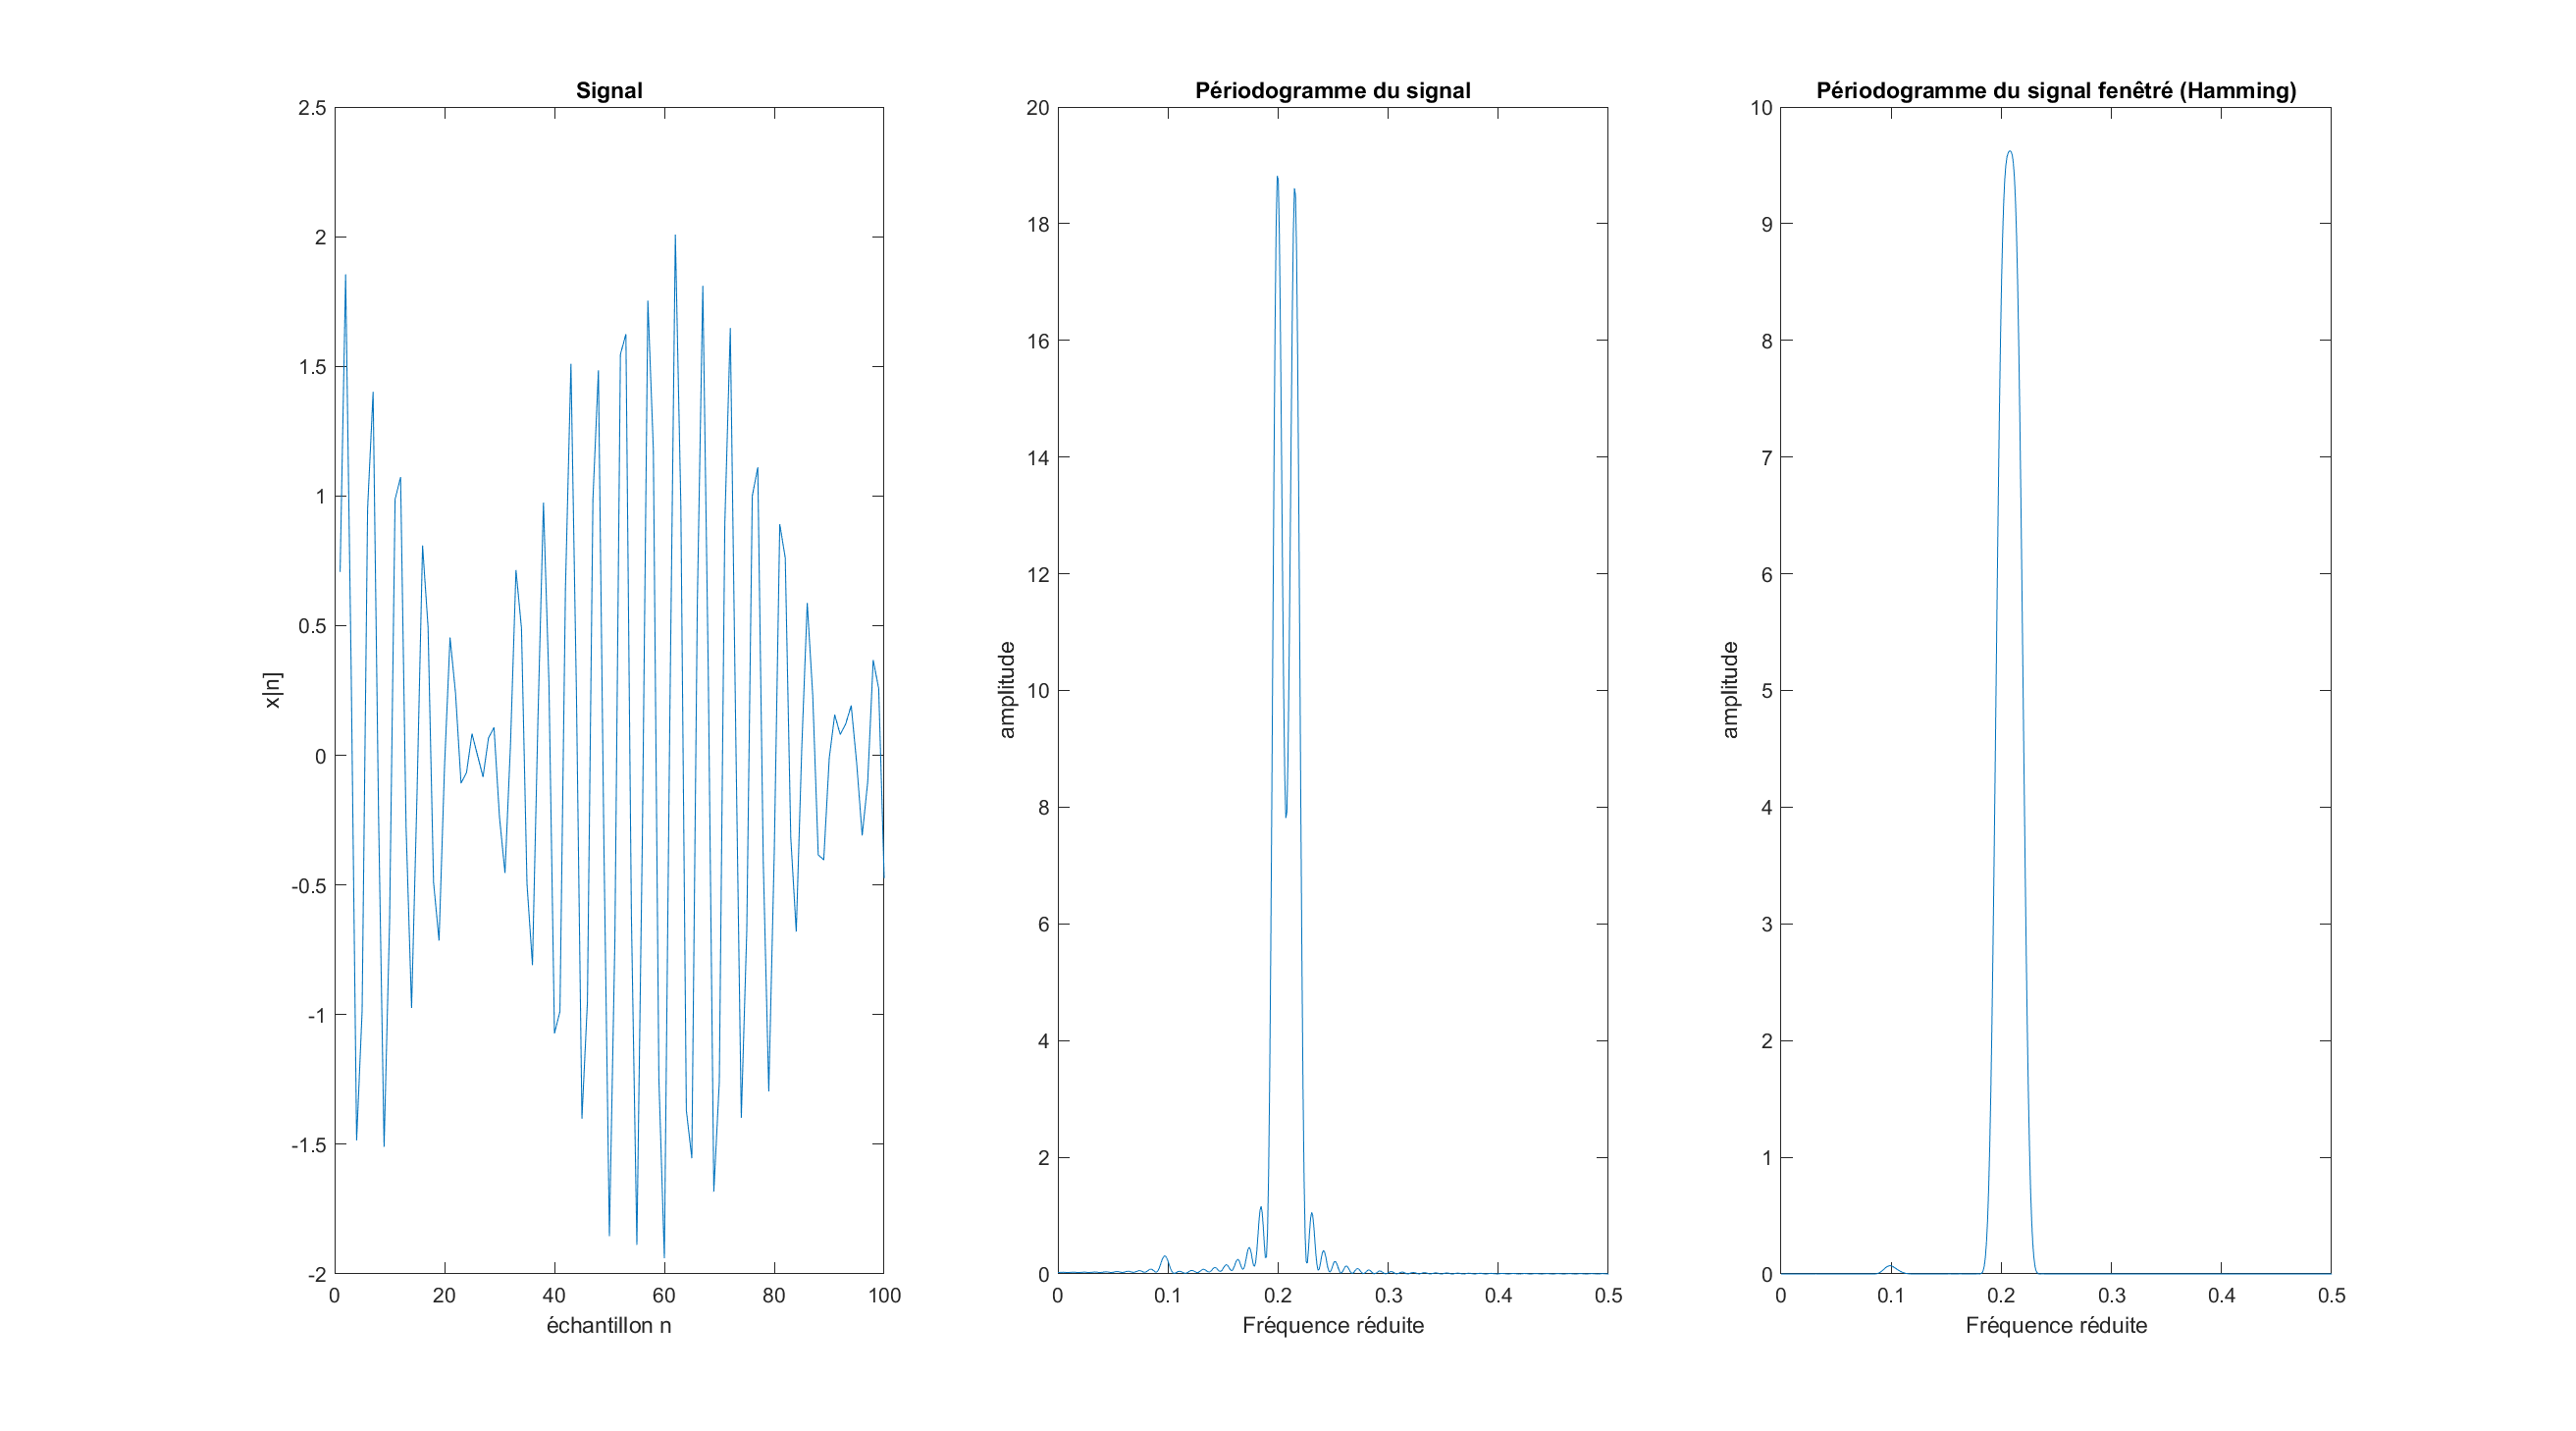
\includegraphics[width=\textwidth]{sig1}
    \centering
\end{figure}

Nous observons que le périodogramme permet d'identifier deux fréquences proches du signal
mais les oscillations semblent cacher une troisième composante. Afin de s'en assurer nous
traçons le périodogramme fenêtré (Hamming) qui permet en limitant la taille des lobes secondaires
de trouver cette troisième composante. Mais le lobe principal ayant alors été élargi nous ne distinguons
plus les deux composantes proches du signal. Nous somme face à un cas illustrant parfaitement la
notion de compromis entre la taille des lobes secondaires et du lobe principal.

En somme le signal 1 semble comporter les composantes : $\lambda_1 = 0.1$, $\lambda_2 = 0.20$ et
$\lambda_3 = 0.21$.

\subsection*{Signal 2}

Pour ce deuxième signal sans bruit, nous optons cette fois pour le calcul du périodogramme, d'un
périodogtramme fenêtré et de la densité spectrale (MUSIC).

En effet, cette fois le périodogramme fenêtré n'est pas suffisant afin d'identifier les composantes
du signal comme le montre le tracé de la densité spectrale permettant d'indentifer une deuxième
composante.

\begin{figure}[H]
    \caption{Résultats signal 2}
    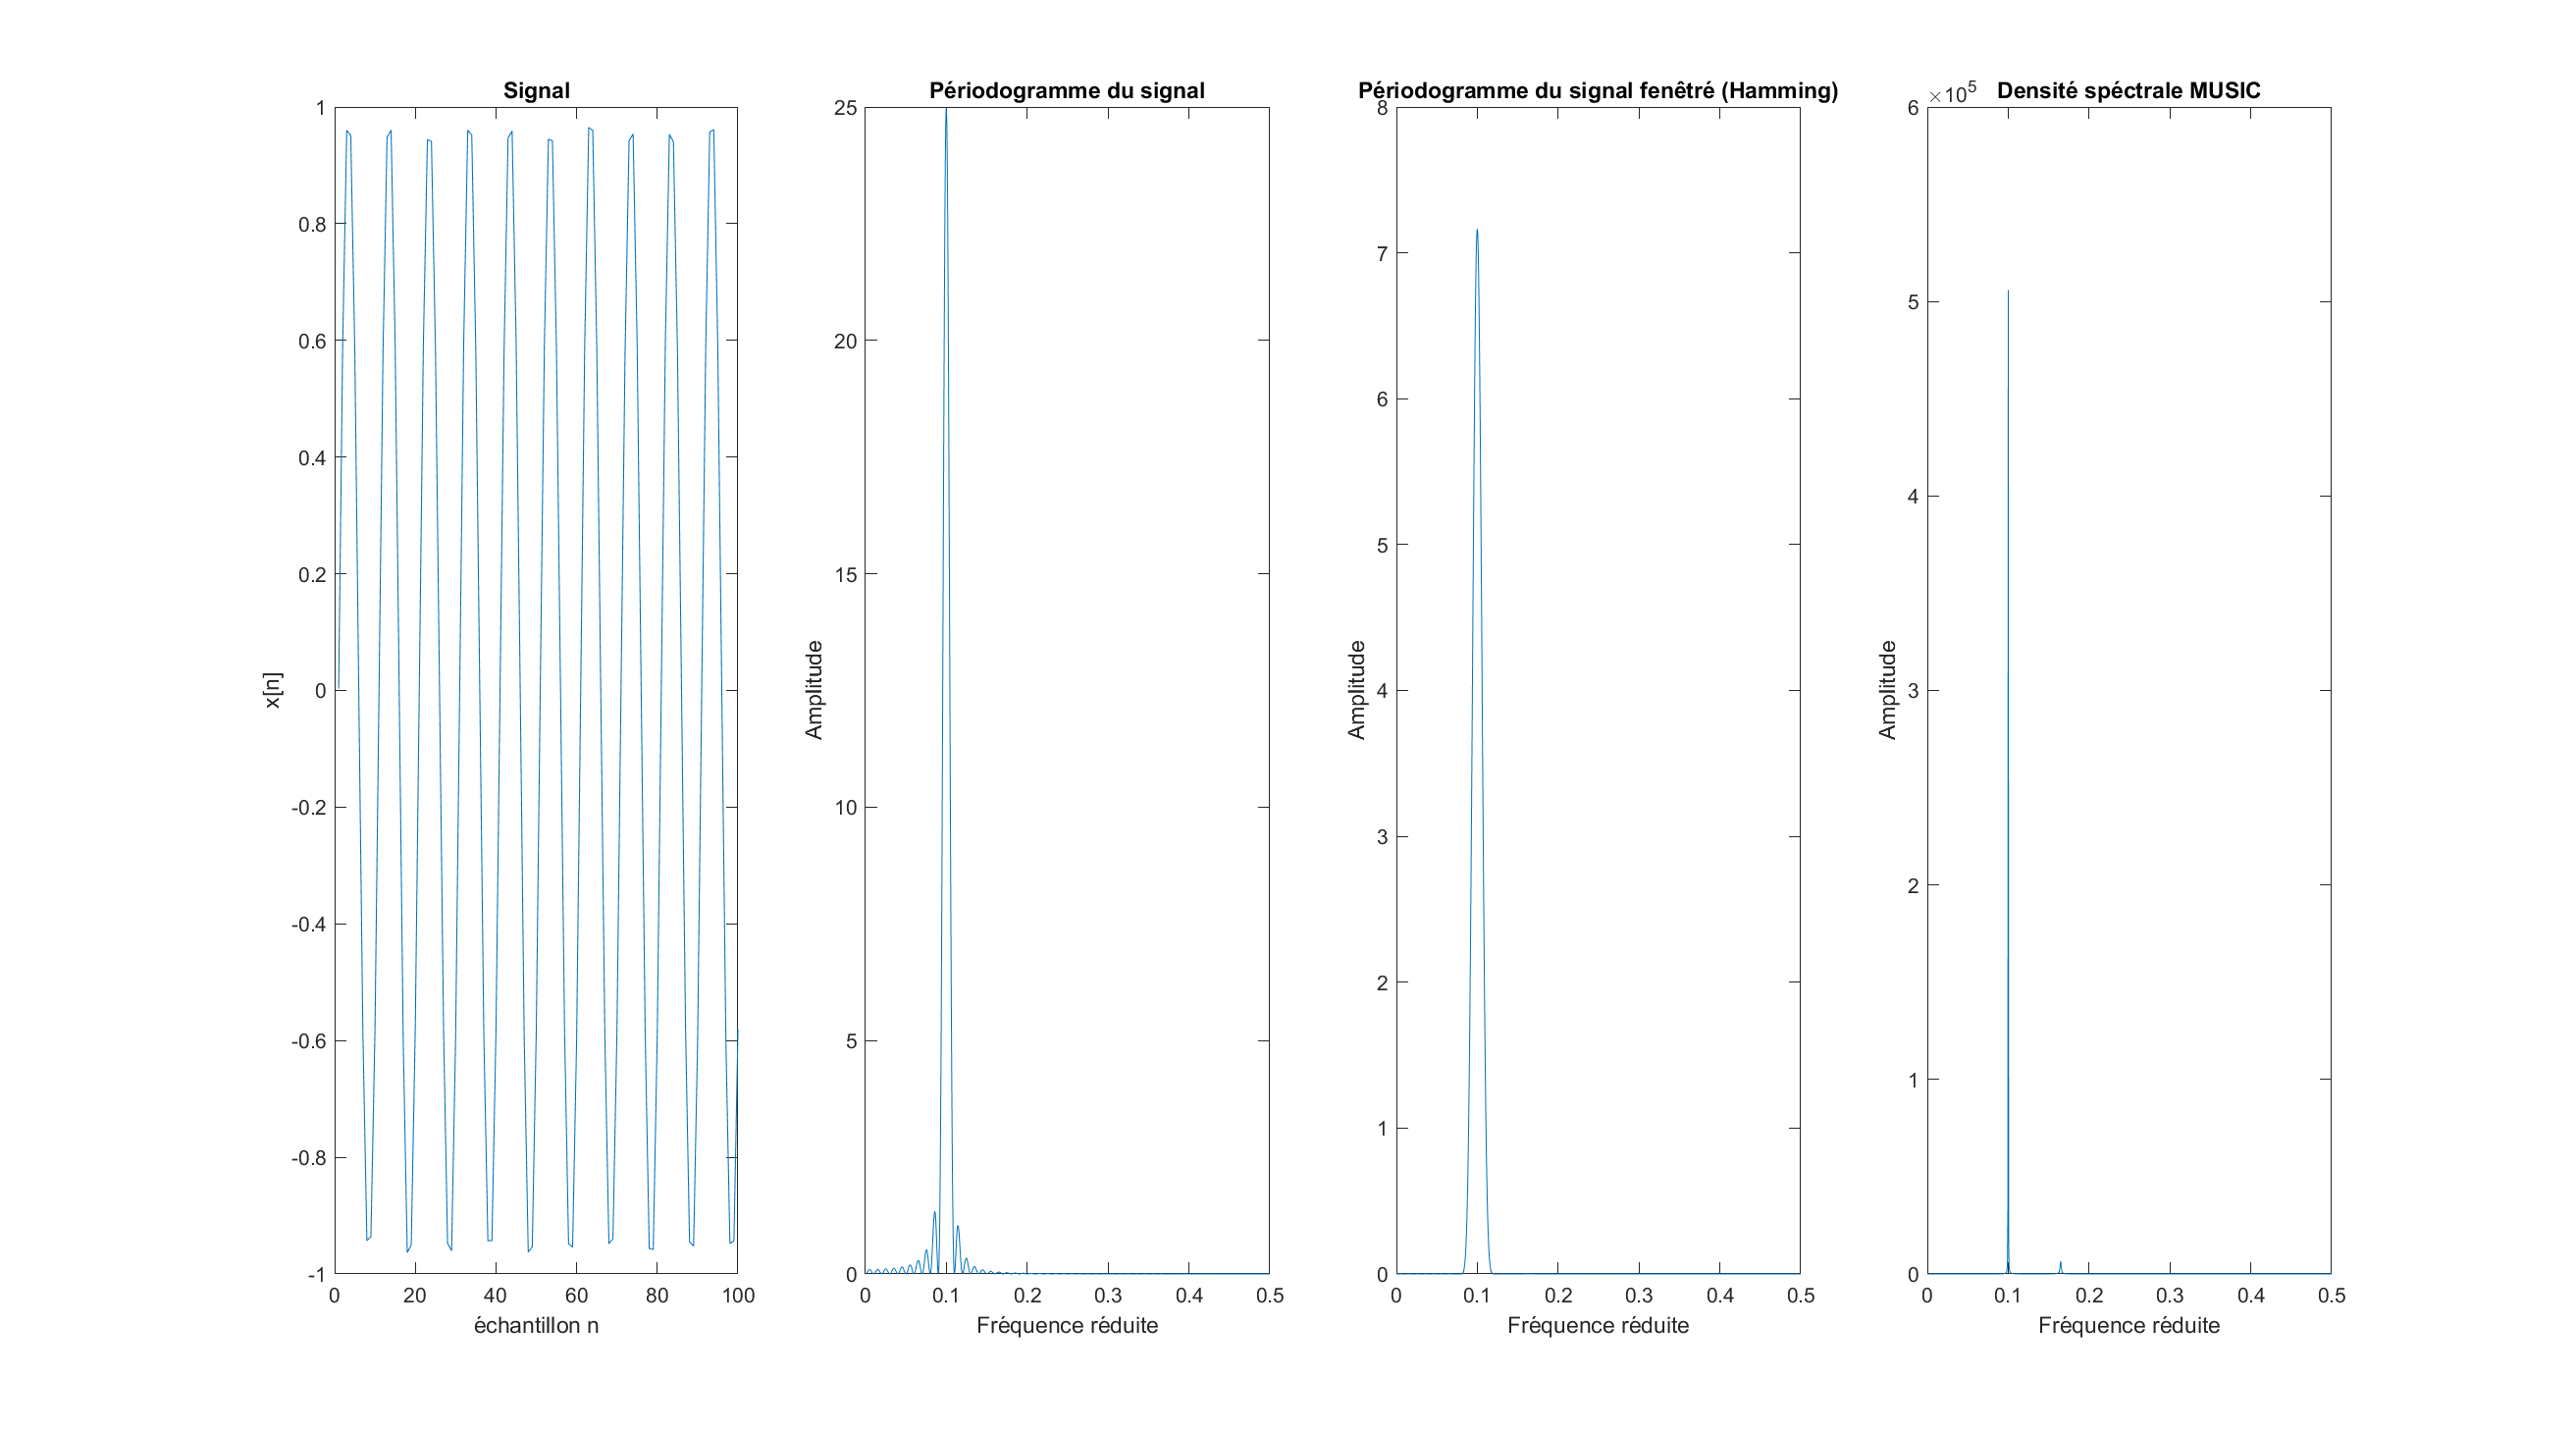
\includegraphics[width=\textwidth]{sig2}
    \centering
\end{figure}

Le signal 2 semble comporter les composantes : $\lambda_1 = 0.1$ et $\lambda_2 = 0.17$.

\subsection*{Signal 3}

Pour ce signal comportant du bruit nous optons pour l'utilisation du pariodogramme, du periodogramme de
Welch et de MUSIC.

Le périodogramme et le périodogramme de Welch ne permettent pas d'idntifier précisément dans ce
cas les composantes du signal. La méthode MUSIC semble fournir les meilleurs résultats mais le choix du
nombre d'exponentielles à rechercher est difficile.

\begin{figure}[H]
    \caption{Résultats signal 3}
    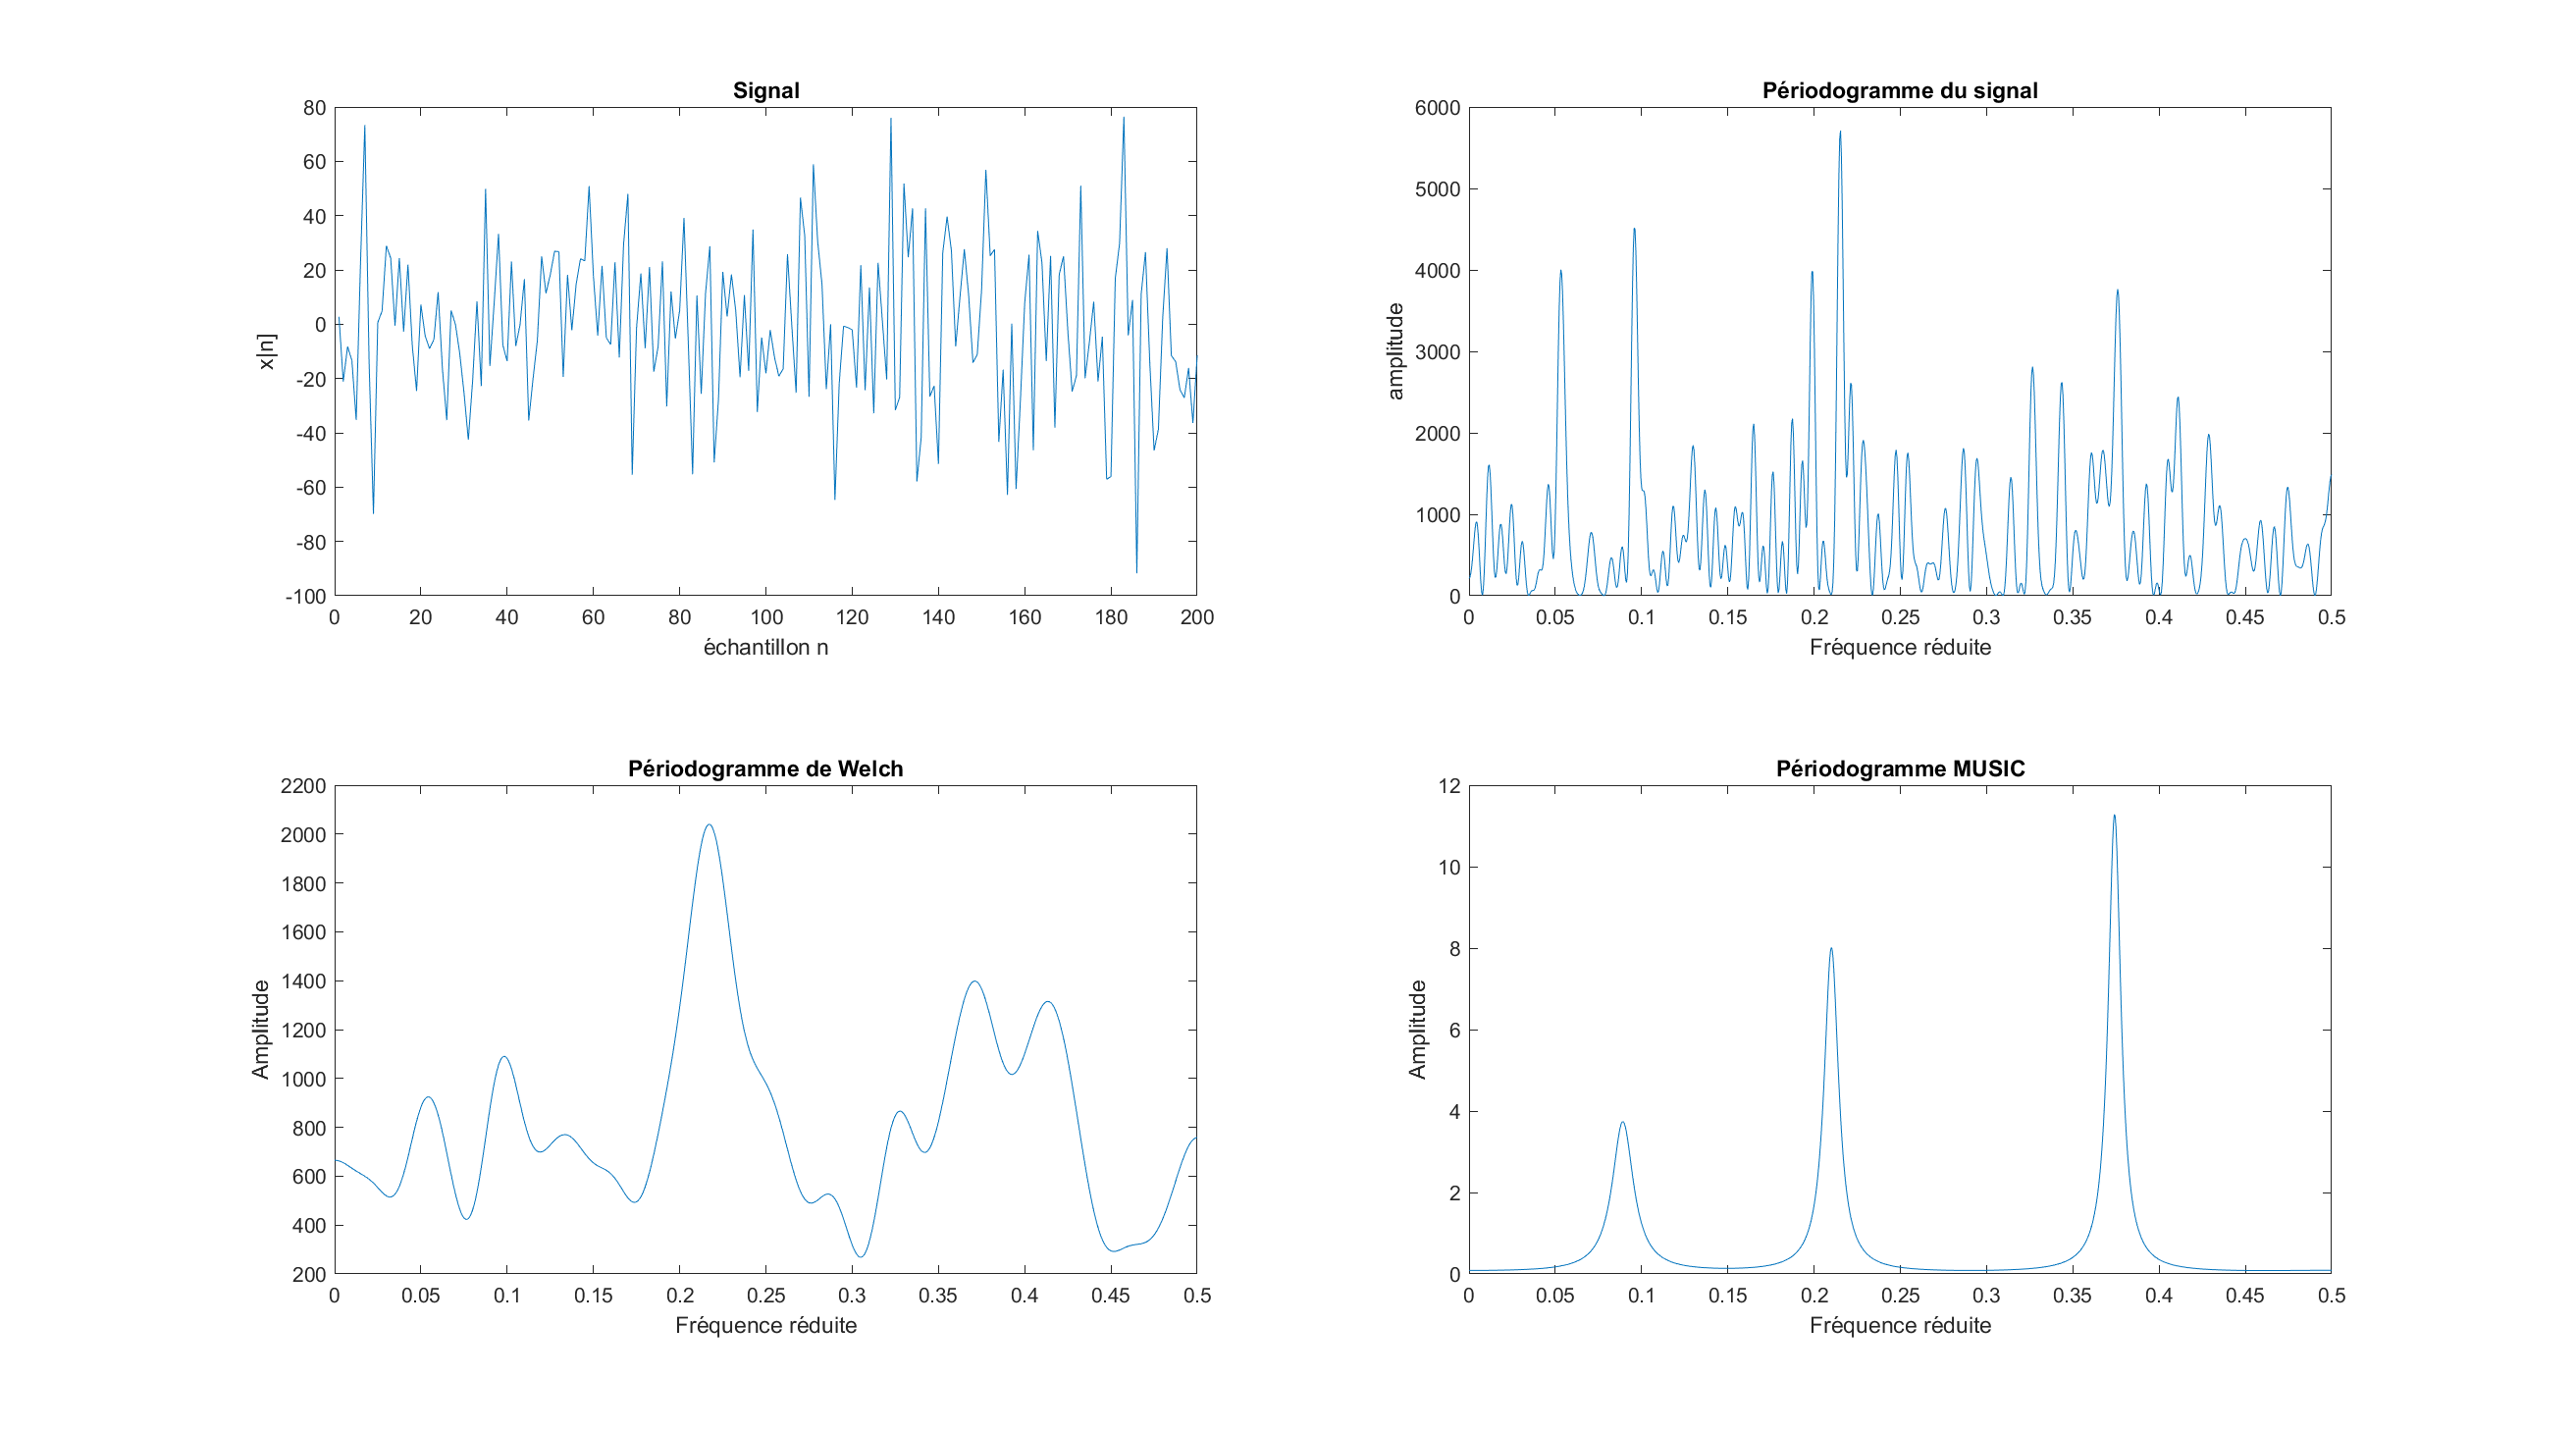
\includegraphics[width=\textwidth]{sig3}
    \centering
\end{figure}

Le signal 3 semble alors comporter les composantes : $\lambda_1 = 0.09$, $\lambda_2 = 0.2$ et
$\lambda_3 = 0.37$.

\subsection*{Signal 4}

Enfin, pour ce dernier signal nous utilisons le périodogramme, MUSIC et la modélisation 
autorégressive.

\begin{figure}[H]
    \caption{Résultats signal 4}
    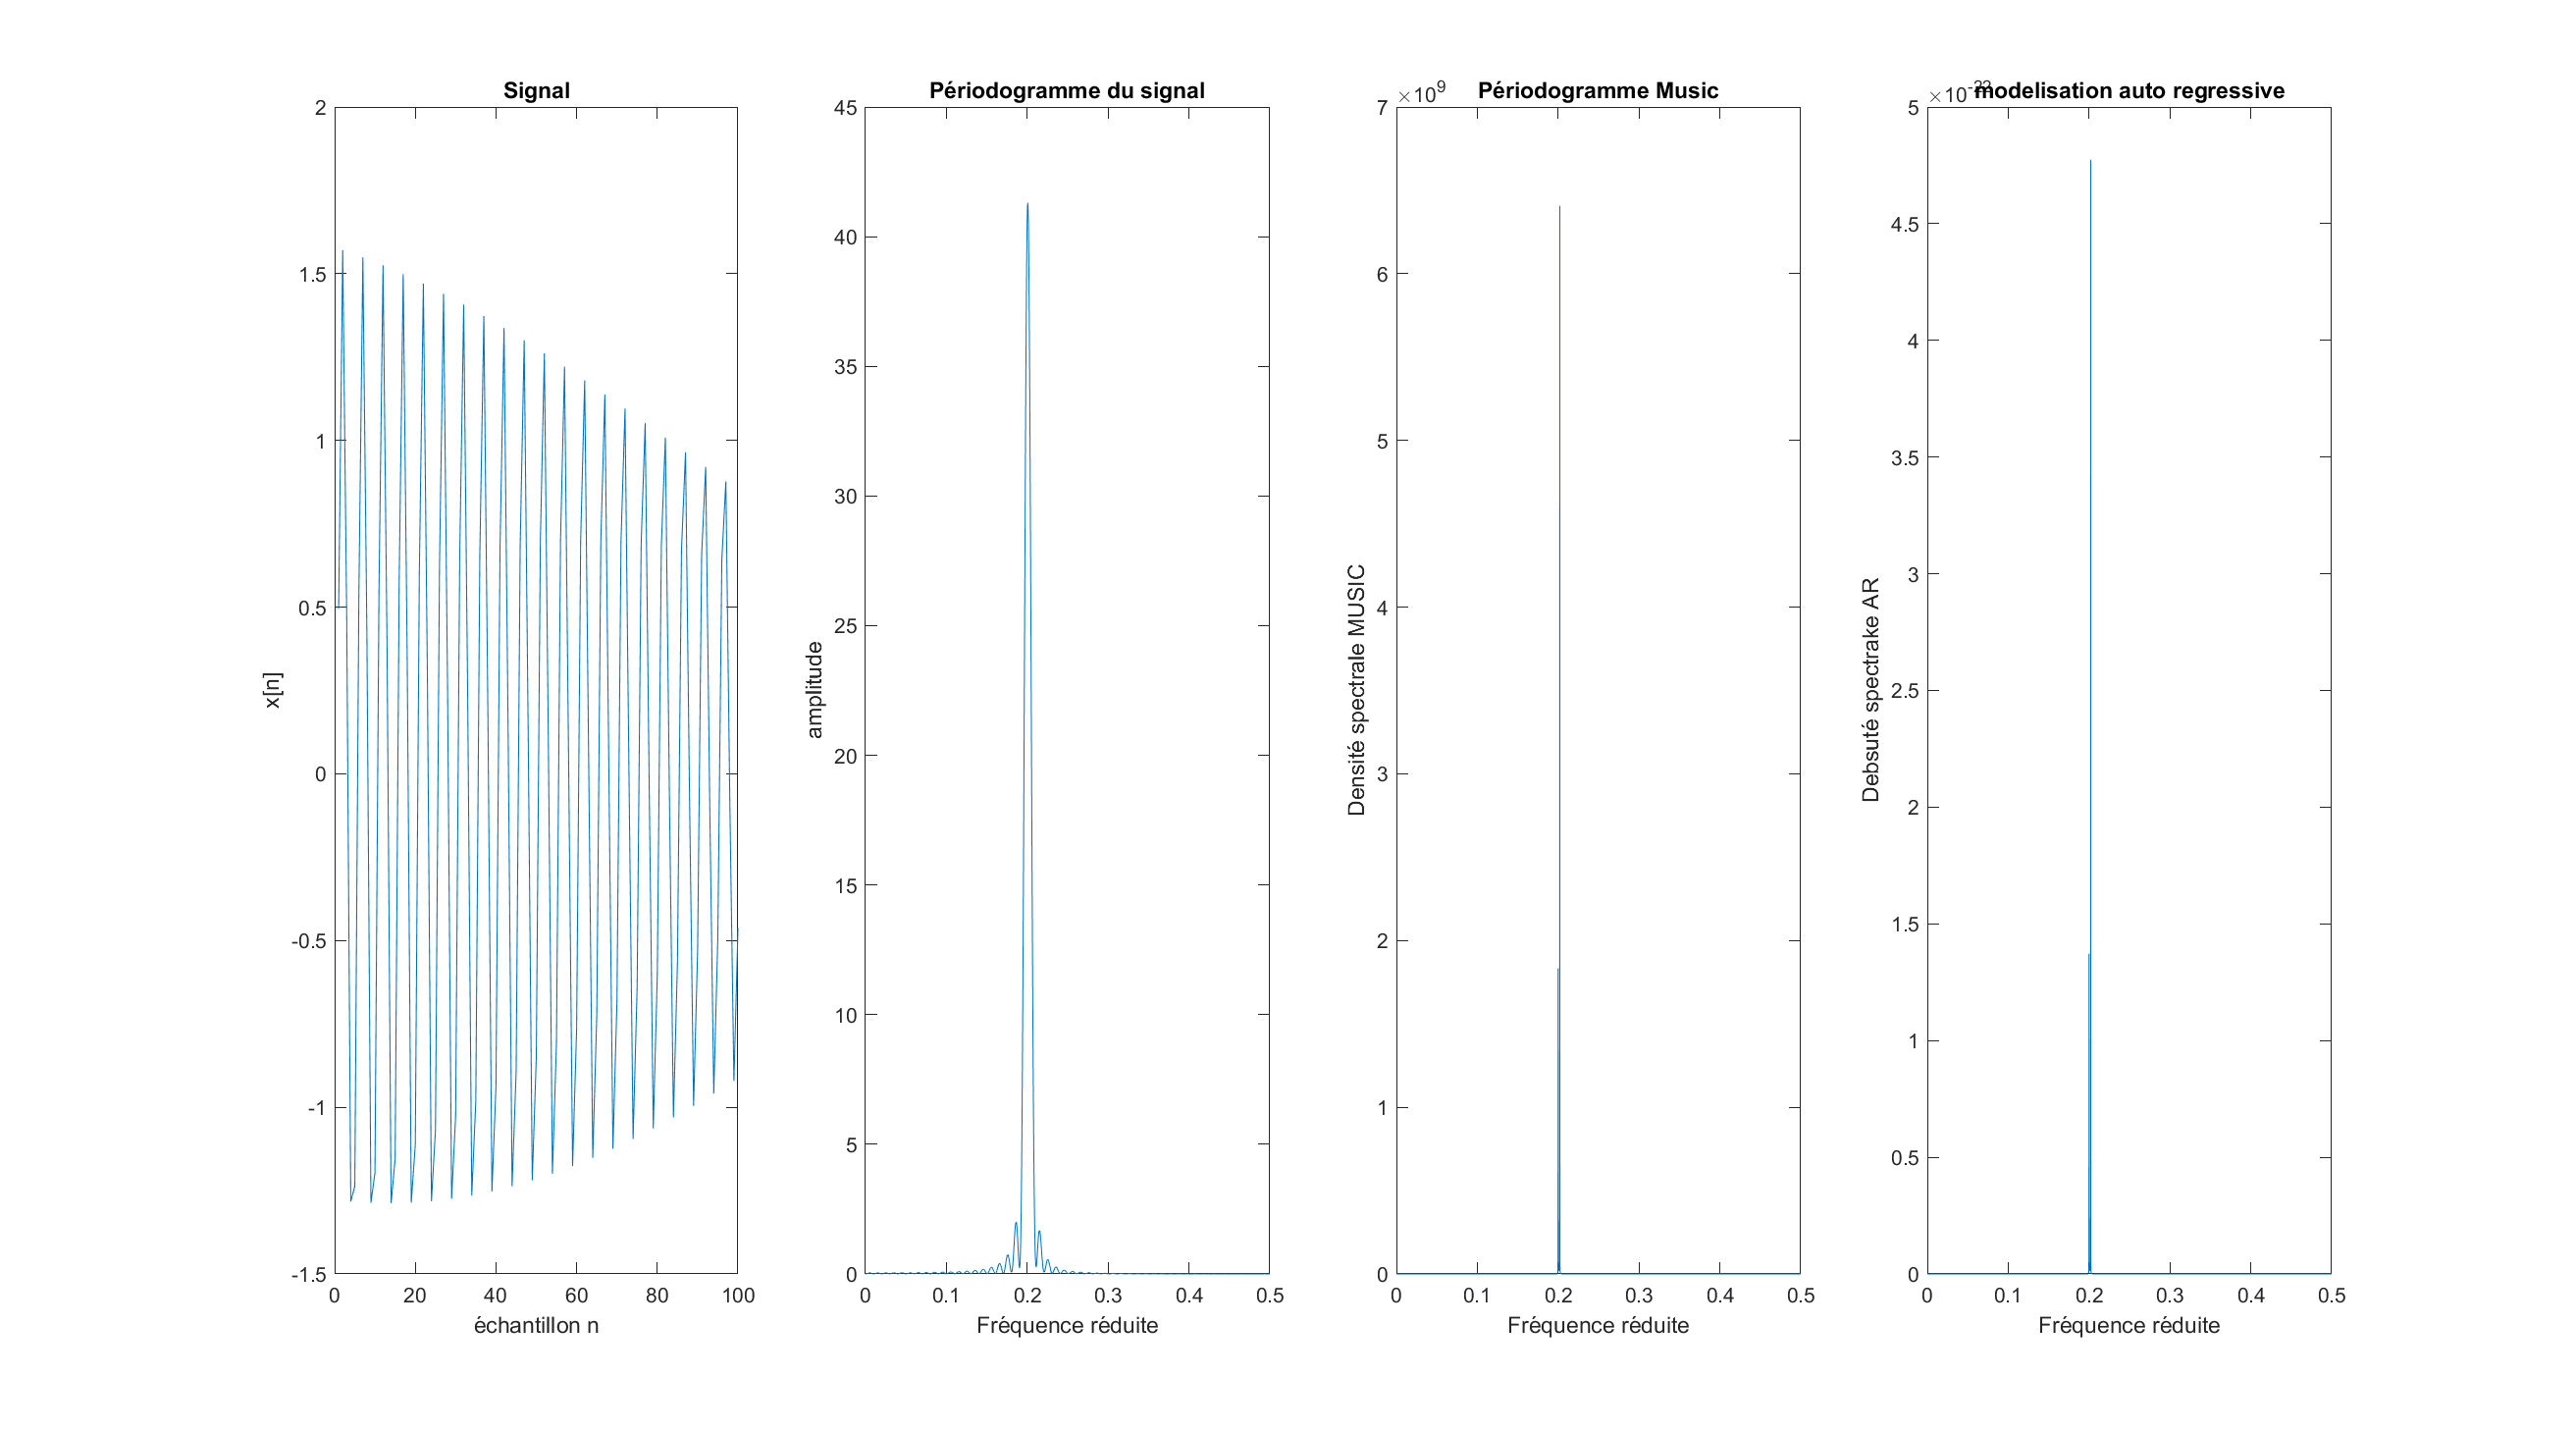
\includegraphics[width=\textwidth]{sig4}
    \centering
\end{figure}

MUSIC et la modélisation autorégressive fournissent alors les meilleurs résultats et permettent
d'identifier deux composantes très proches du signal.

Le signal 4 semble alors comporter les composantes : $\lambda_1 = 0.199$ et $\lambda_2 = 0.2$.

\subsection*{Résumé des avantages et limites de chaque méthode}

D'après les résultats précedents on retiendra ces avantages et limites des différentes méthodes
d'analyse spectrale présentées :

\begin{table}[h]
    \begin{tabularx}{\textwidth}{ |l|X|X| }
        \hline
        Méthode & Avantages & Inconvénients \\
        \hline
        Périodogramme & Bonne estimation du lobe principal & Masquage des composantes de faibles amplitudes \\
        \hline
        Périodogramme fenêtré & Meilleure estimation des composantes de faibles amplitudes & étalement du lobe principal \\
        \hline
        Périodogramme de Welch & Réduction de l'influence du bruit & perte de l'hypothèse de stationnarité si recherche d'une meilleure résolution \\
        \hline
        Modélisation autorégressive & Réduction de l'influence du bruit, méthode paramétrique & Couteux en calculs, méthode asymptotique \\
        \hline
        MUSIC & adapté à une utilisation en présence de bruit & Couteux en calculs, méthode asymptotique, choix d'un paramètre \\
        \hline
    \end{tabularx}
\end{table}

\section{Détection d'exoplanètes par analyse spectrale de série temporelle}

\begin{enumerate}

    \item[1.] 
        Représentons la transformée de fourier en module de la fenêtre d'observation :

        \begin{figure}[H]
            \caption{Fenêtre d'observation}
            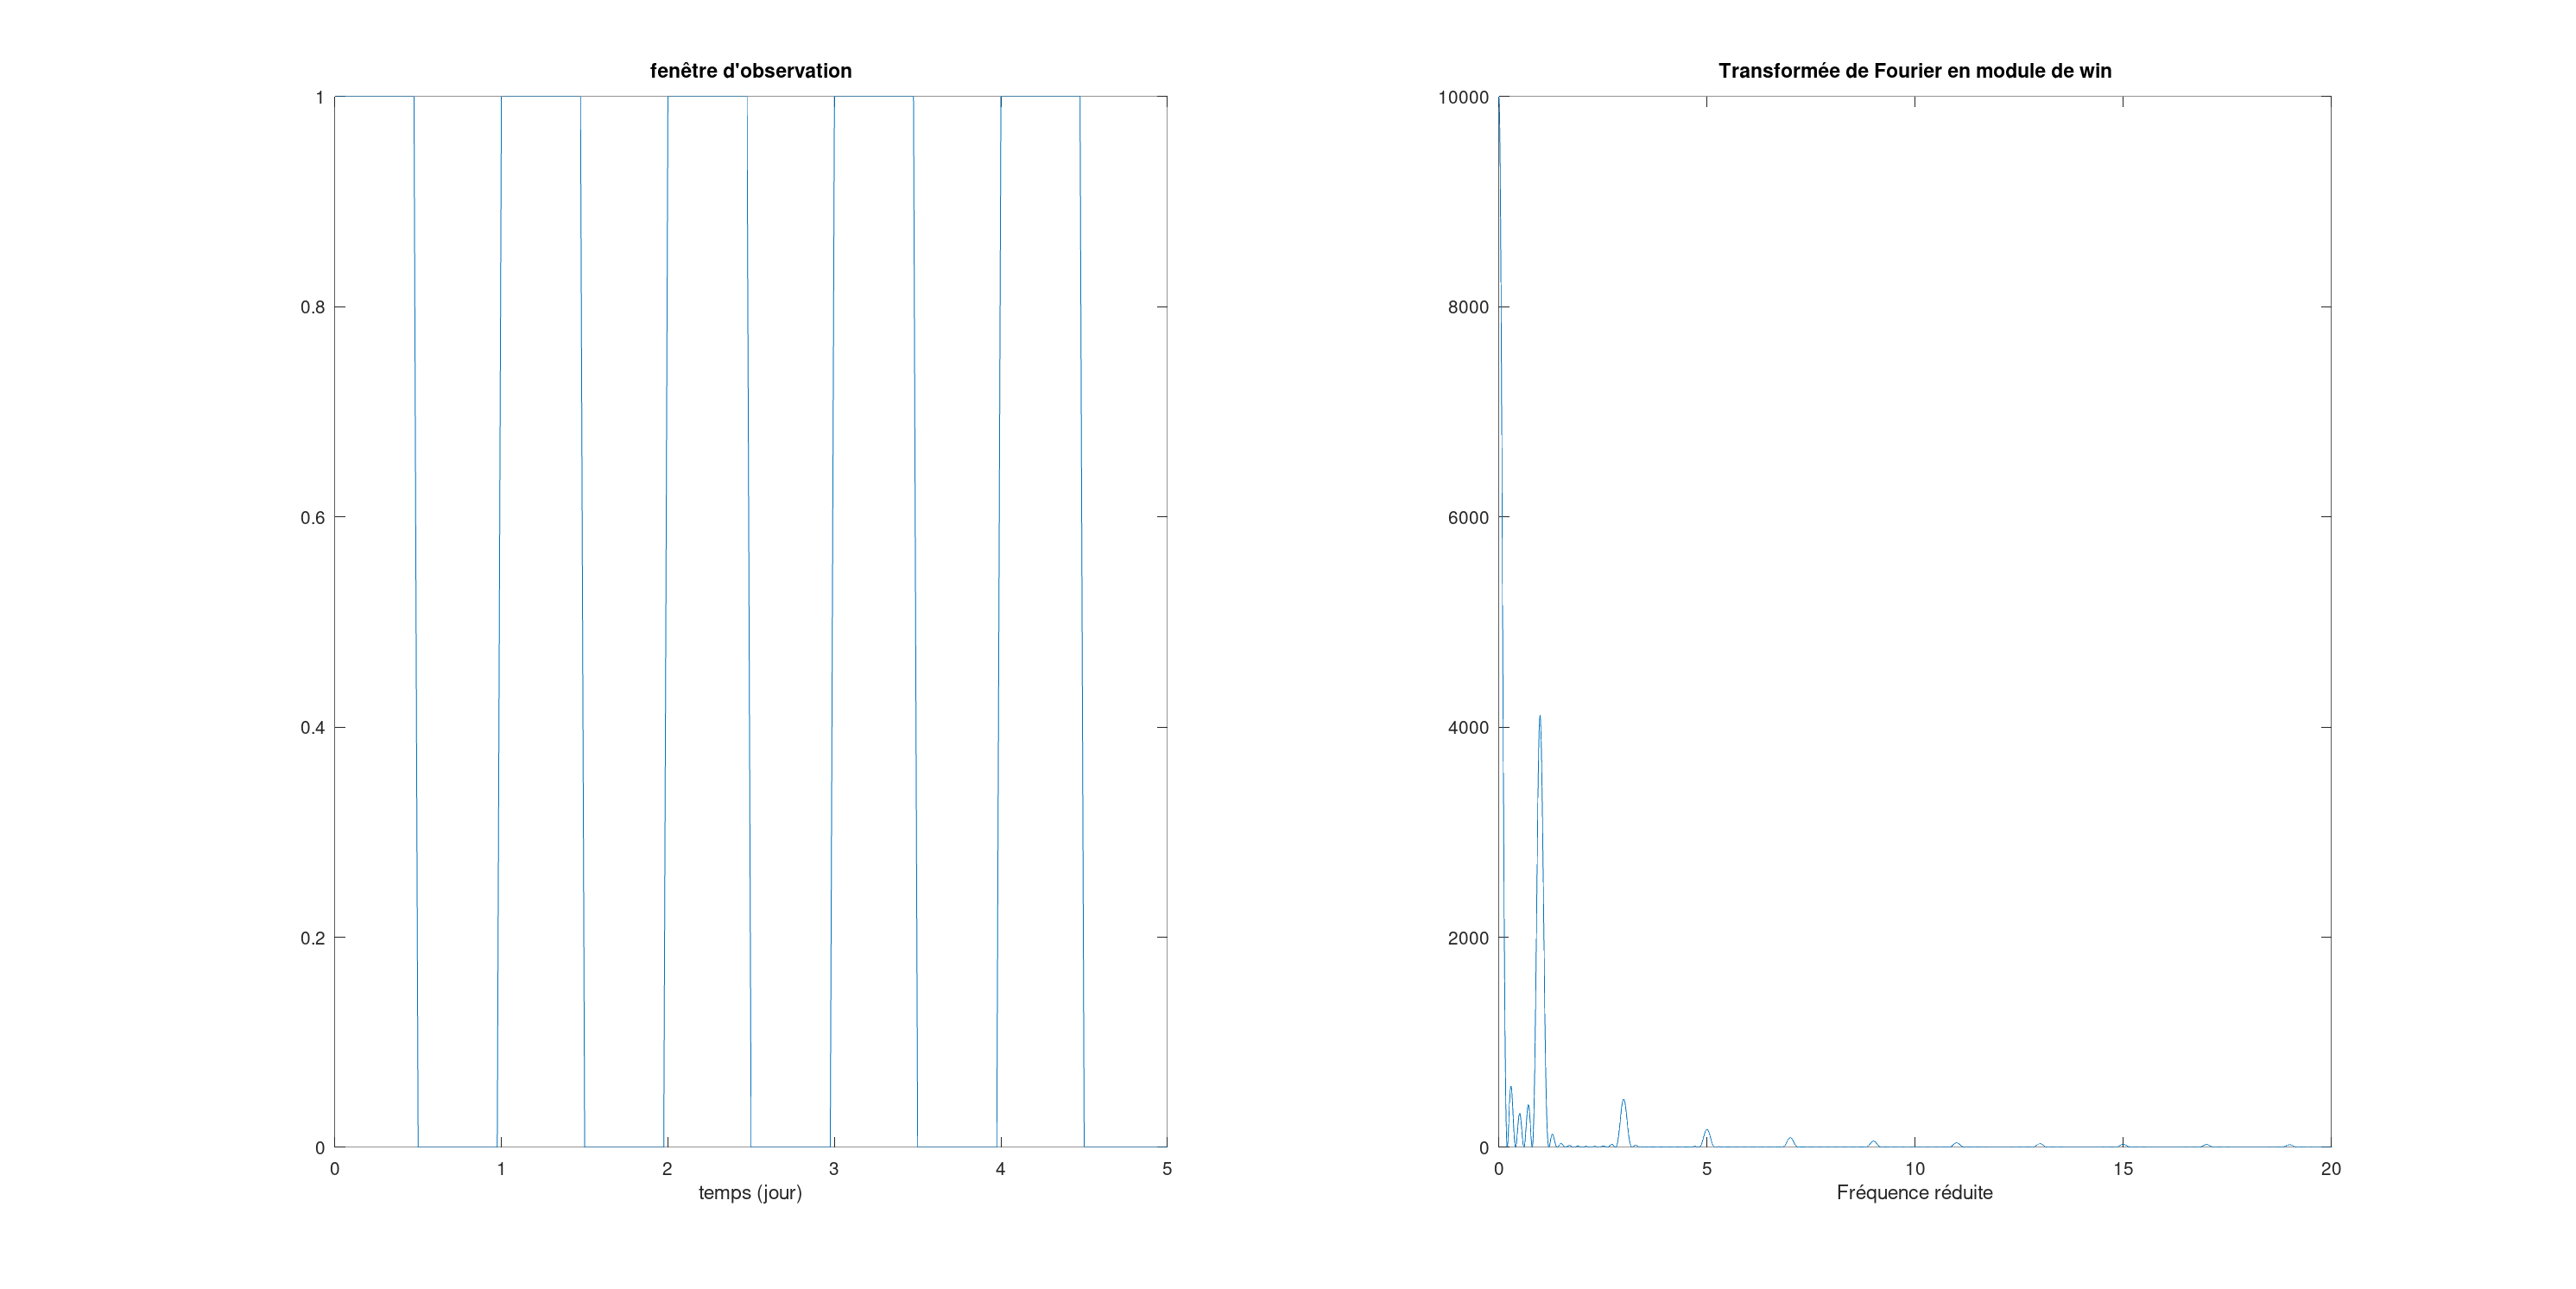
\includegraphics[width=\textwidth]{win}
            \centering
        \end{figure}

    Ce périodogramme met alors en évidence l'ajout de bruit au périodogramme du signal.

    \item[2.] 
        Représentons le périodogramme du signal :

        \begin{figure}[H]
            \caption{Signal (données disponibles}
            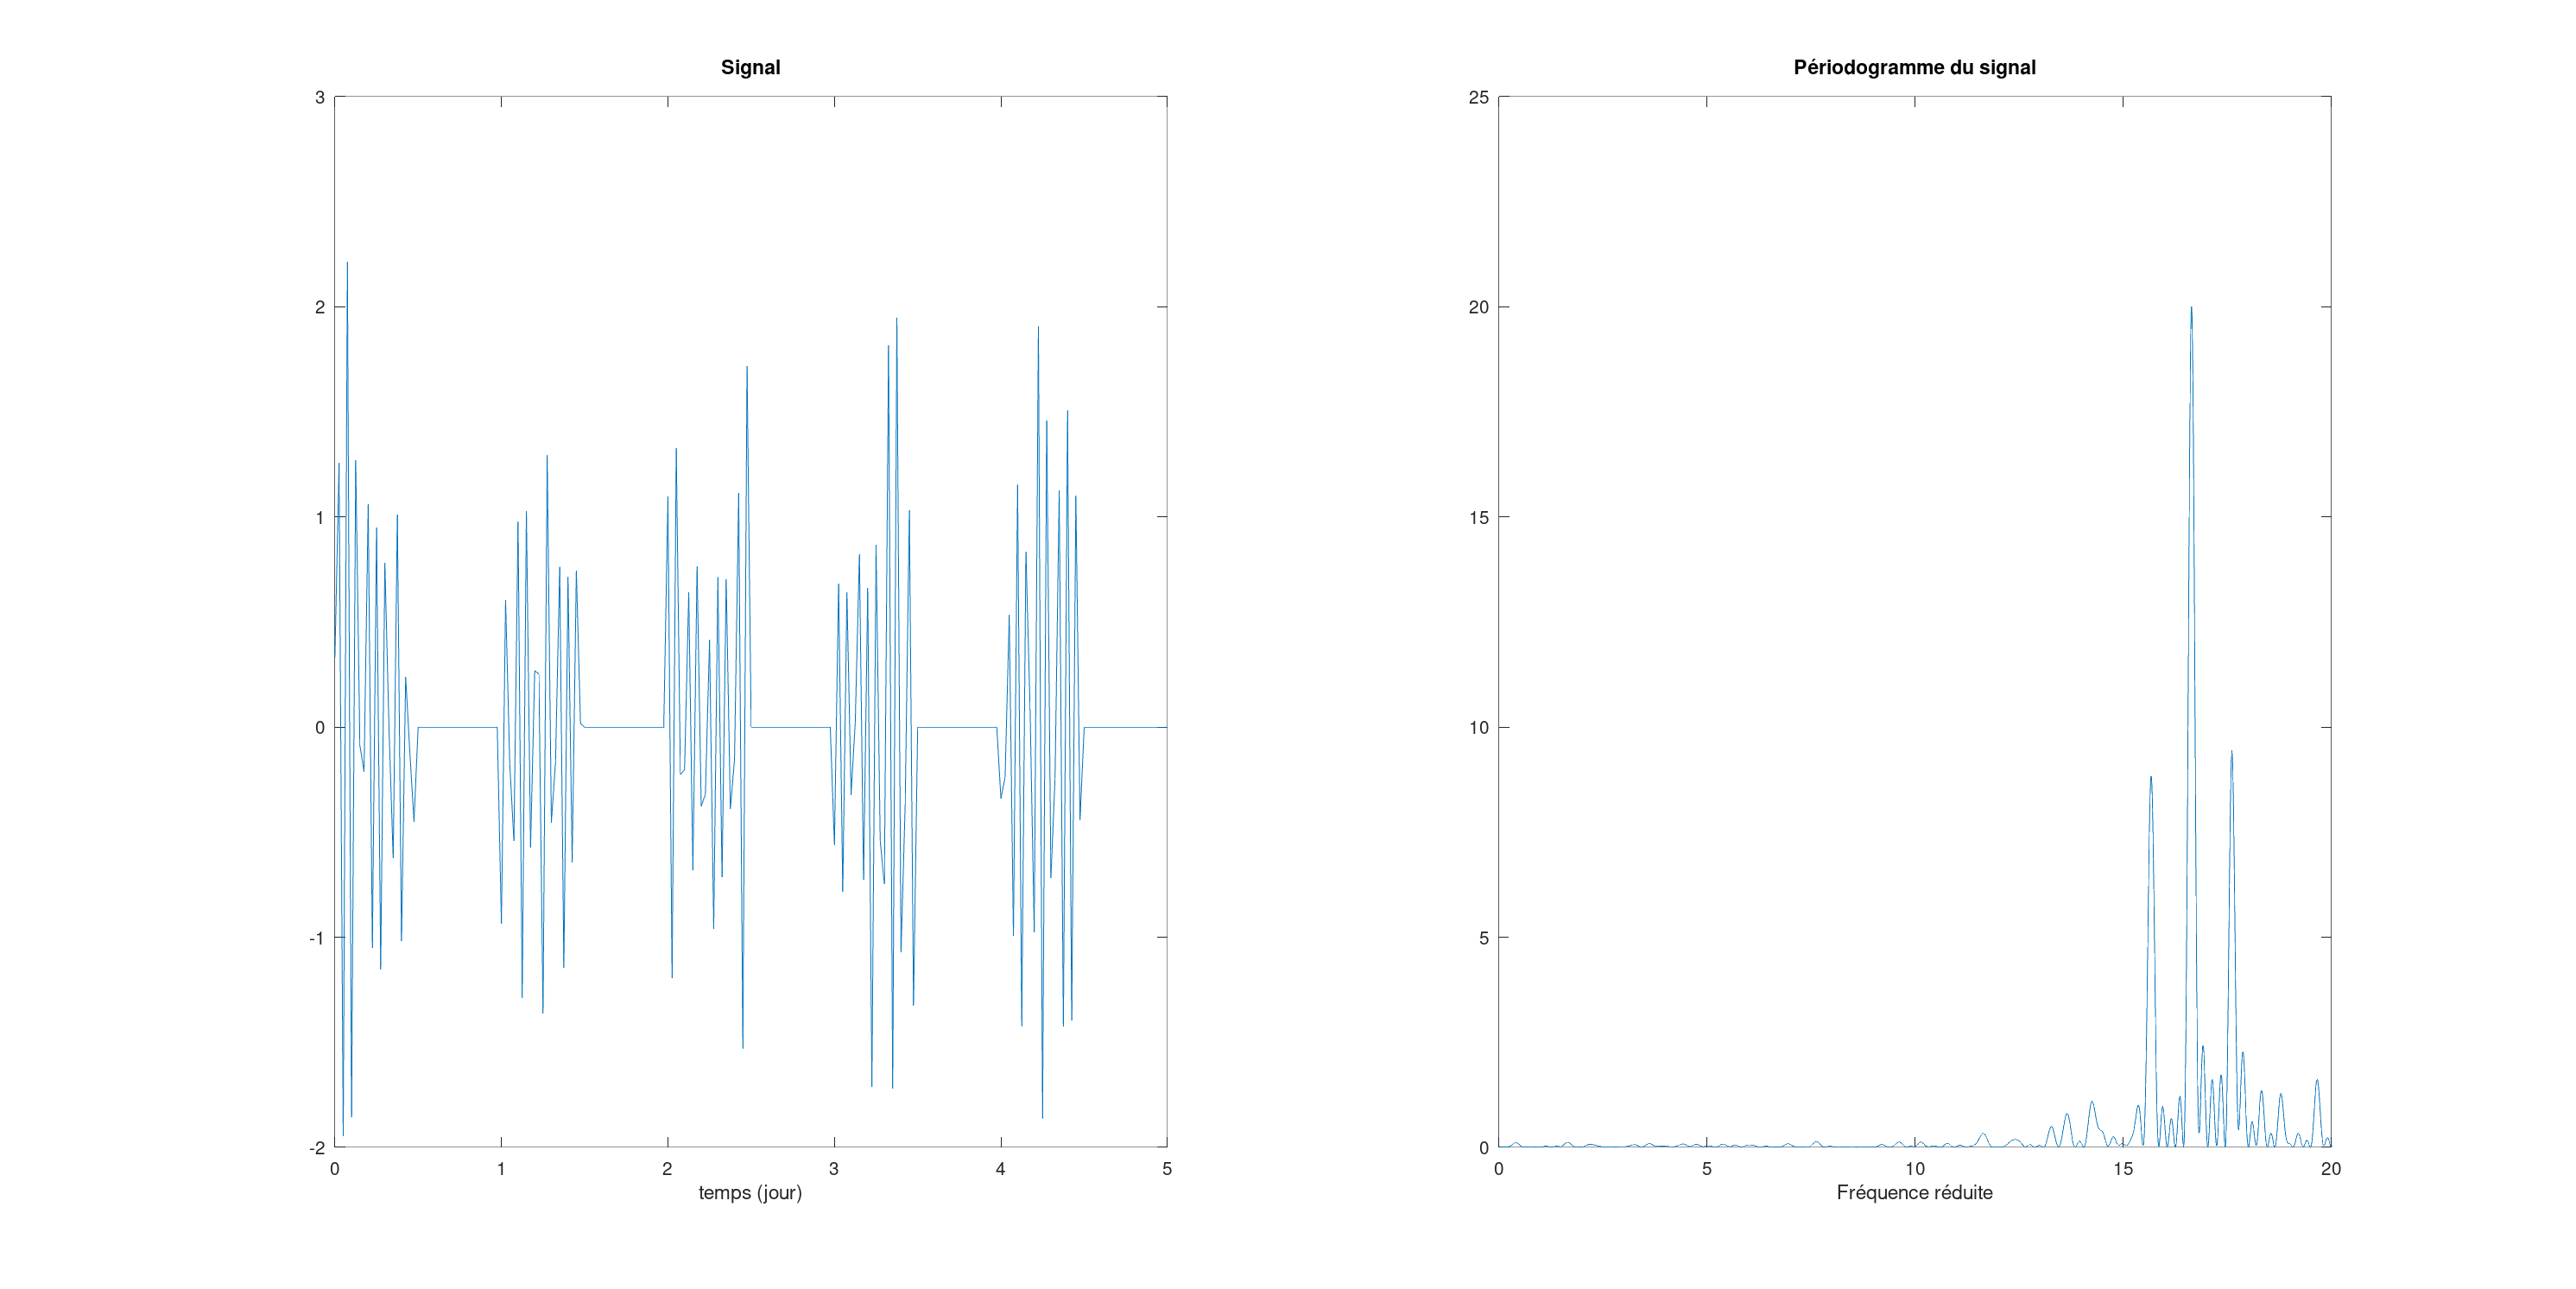
\includegraphics[width=\textwidth]{periodogramme_sig}
            \centering
        \end{figure}

    On observe que le périodogramme contient en plus de l'information utile du bruit.
    Il faudra alors procéder à une étape d'isolation de l'information.

    \item[3.] 

        L'implémentation de l'algorithme présenté est fournie en Annexe.

    \item[4.] 

        En faisant tourner l'algorithme on obtient les résultats suivants pour les 3 premières
        itérations de l'algorithme : 

        \begin{figure}[H]
            \caption{Itération 1}
            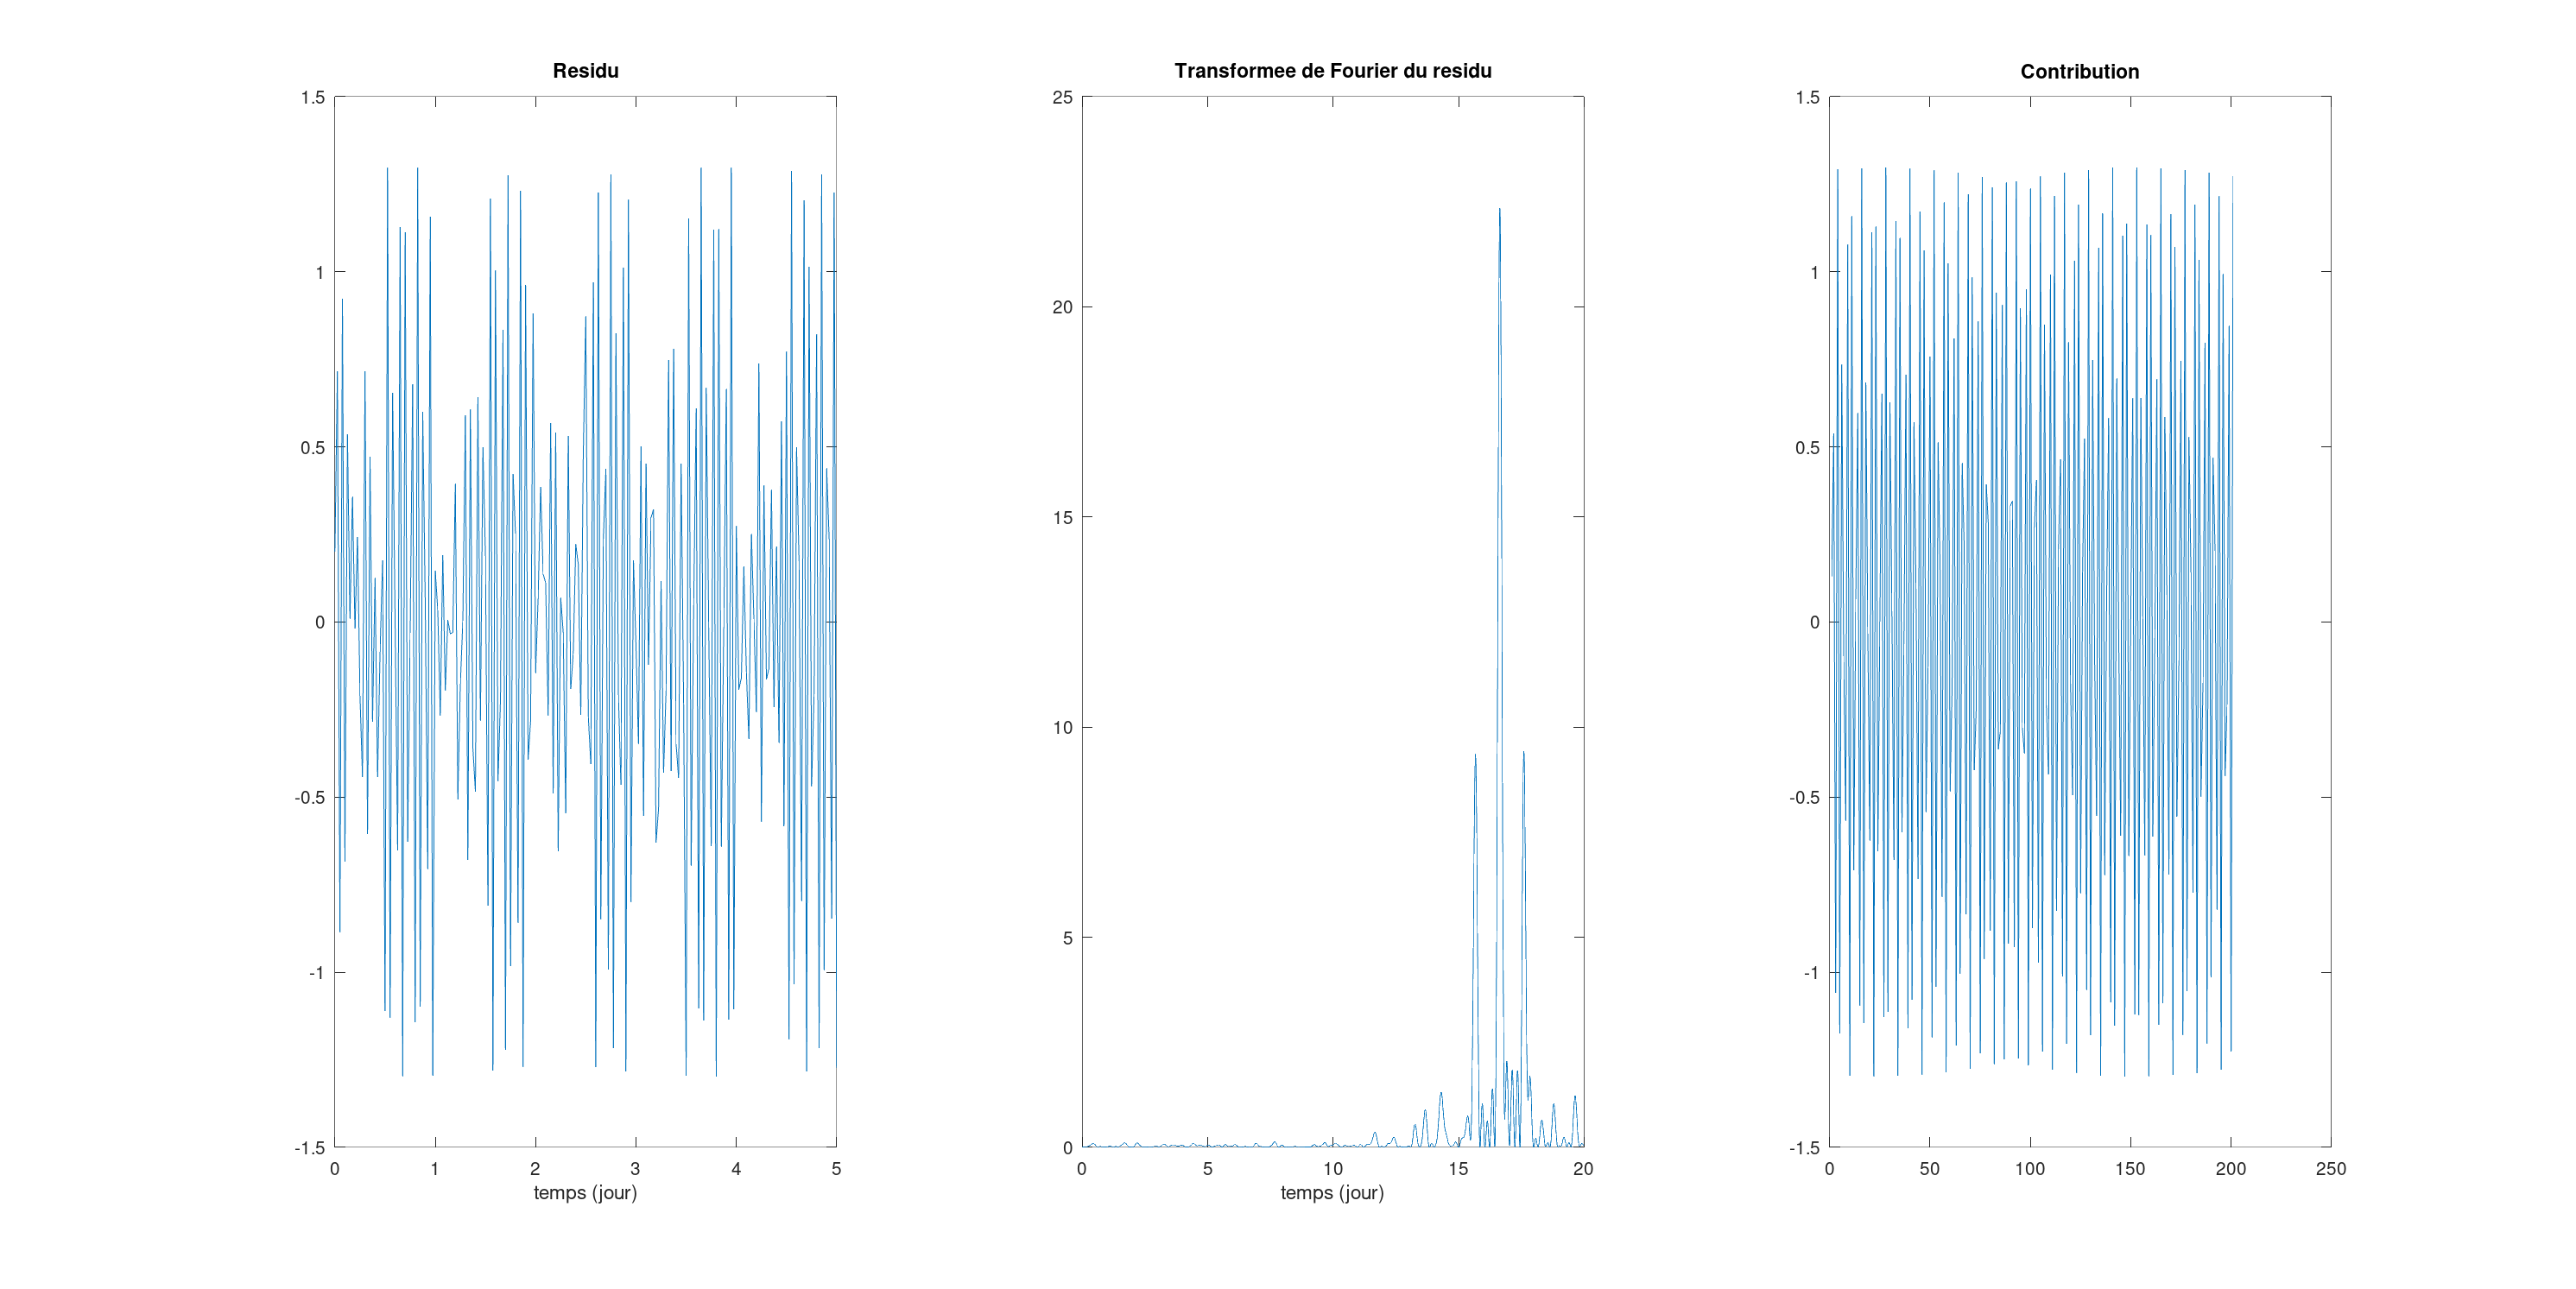
\includegraphics[width=\textwidth]{iter1}
            \centering
        \end{figure}

        \begin{figure}[H]
            \caption{Itération 2}
            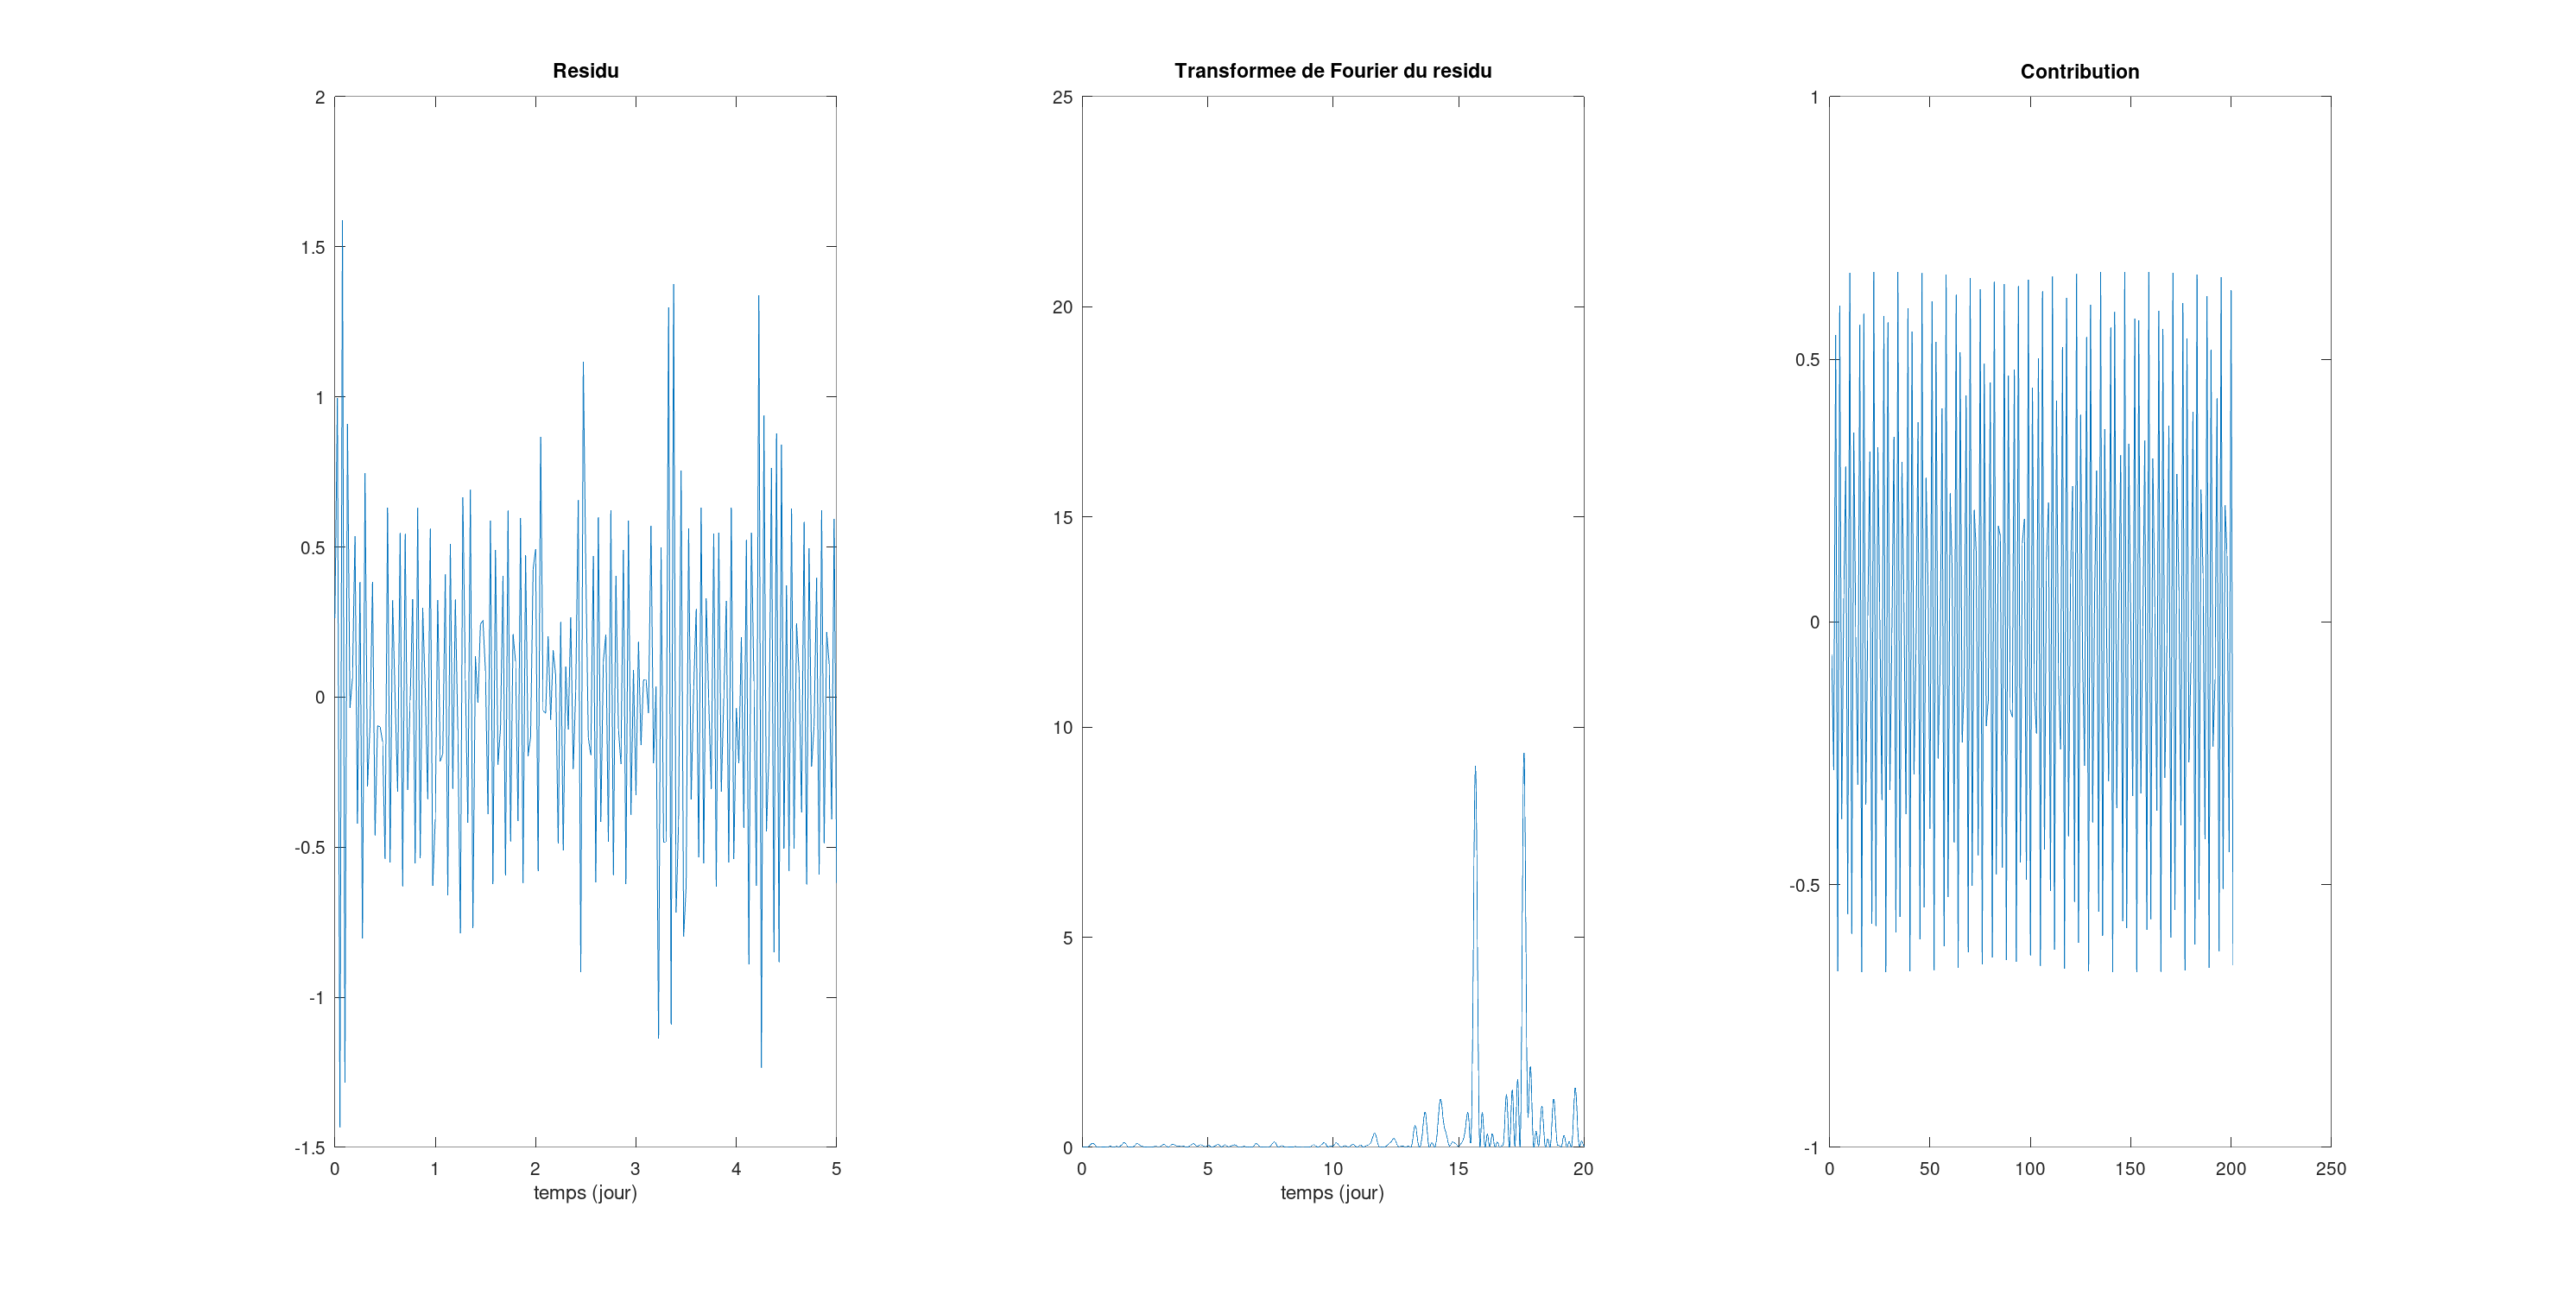
\includegraphics[width=\textwidth]{iter2}
            \centering
        \end{figure}

        \begin{figure}[H]
            \caption{Itération 3}
            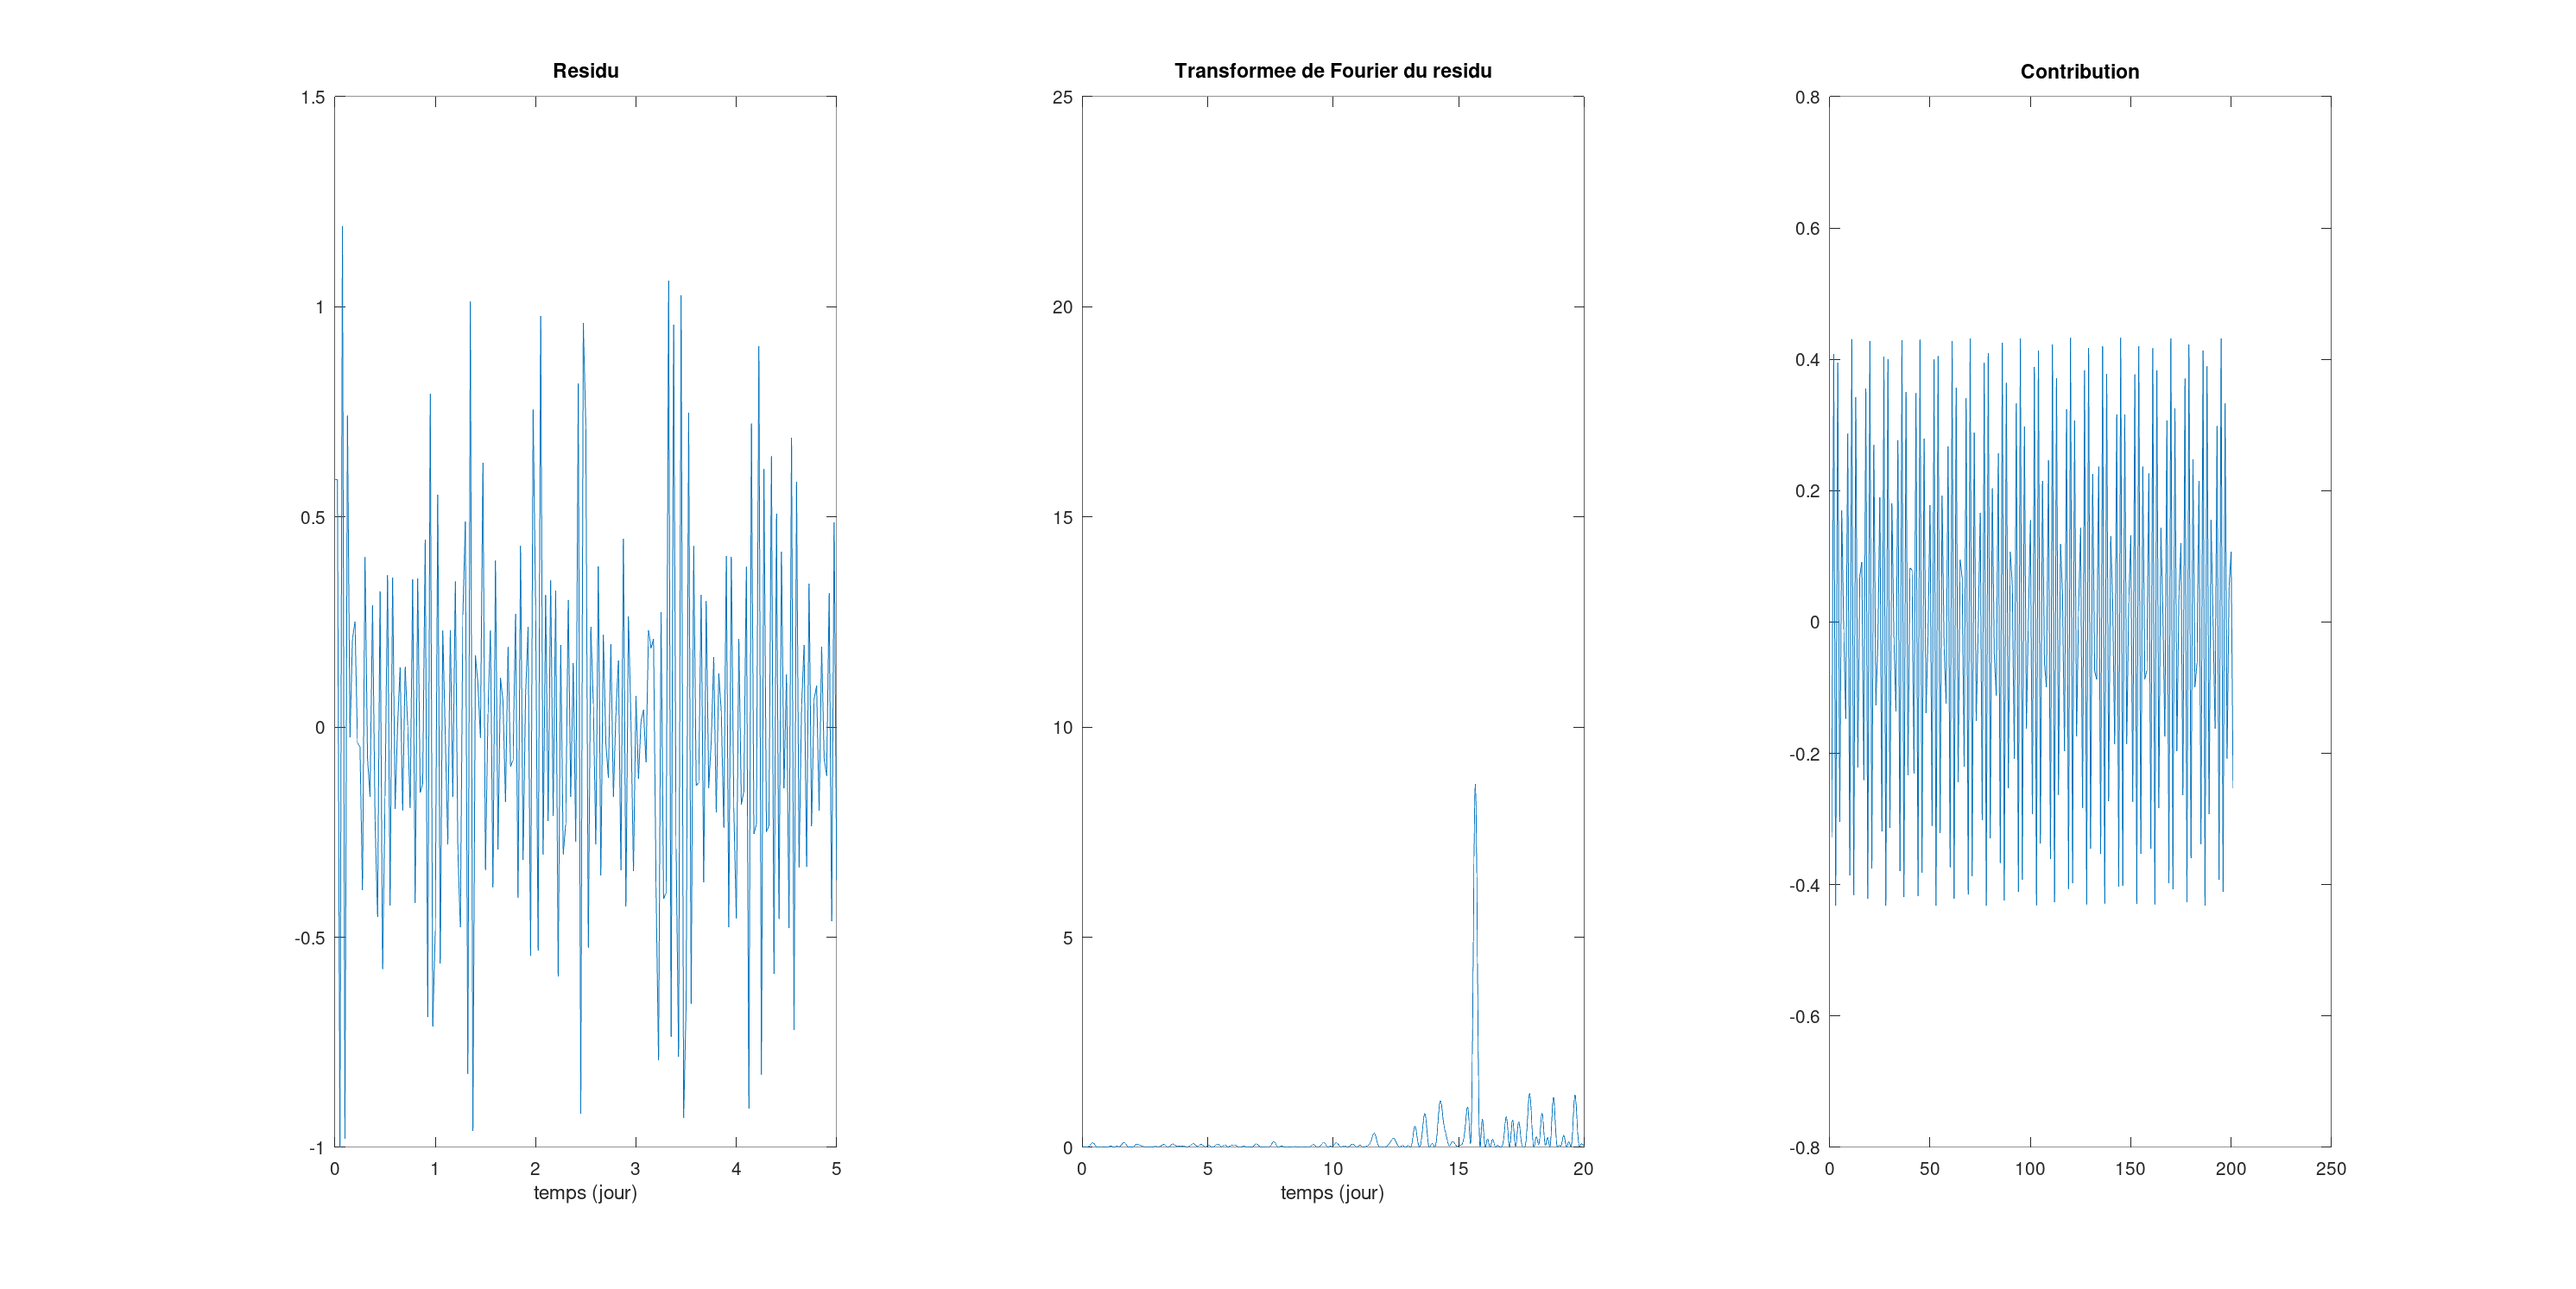
\includegraphics[width=\textwidth]{iter3}
            \centering
        \end{figure}

        Ainsi, on observe que la méthode permet bien de détecter les composantes du signal, à
        chaque itération la composante correspondant à l'amplitude la plus importante est éliminée.
        On dispose alors d'une nouvelle méthode, cette fois itérative d'extraction des composantes
        fréquentielles d'un signal en présence de pics parasites.

\end{enumerate}

\begin{appendices}

    \section{Script Signal 1}

    \lstinputlisting[language=Matlab]{../signal1.m}

    \section{Script Signal 2}

    \lstinputlisting[language=Matlab]{../signal2.m}

    \section{Script Signal 3}

    \lstinputlisting[language=Matlab]{../signal3.m}

    \section{Script Signal 4}

    \lstinputlisting[language=Matlab]{../signal4.m}

    \section{Script Exercice 2}

    \lstinputlisting[language=Matlab]{../astro.m}

\end{appendices}

\end{document}
